\documentclass[11pt]{article}

\usepackage[english]{babel} 
\usepackage{amsmath}
\usepackage{graphicx} 
\usepackage[margin=1in]{geometry}

\title{Simple Grammar Analyzer \\ Max Marchuk}
\author{CS311 Fall 2014}
\date{December 6, 2014}
\begin{document}
\maketitle

\section*{Writeup}

\subsection*{Encoding the Grammar}
\paragraph{}The method that I chose to encode my Grammars was in JSON format. The only structures I really needed for encoding a grammar is a dictionary that maps the variables/symbols to their rules, but I chose to include some additional information such as the start variable (arguably unnecessary, but included anyways) and a short description of the grammar. The criteria for defining my grammars was as follows:
\begin{enumerate}
        \item All rules in the grammar must have a terminal as the first 
        symbol on the right hand side of the rule.
        \item No variable in the grammar can have two rules with the same terminal
        as the first symbol on the right hand side.
    \end{enumerate}
The grammars that I encoded are the following: 
    \[ \{ a^n\#b^n \;|\; n > 0 \} \]
    \[ \{ w\#w^R \;|\; w \in \{0,1\}^* \} \]
    \[ \{ a^i\#b^j\#c^k\# \;|\; i = j \text{ and } i,j,k > 0 \} \]
\paragraph{}I also encoded a grammar that recognizes strings that are valid, single-term algebraic expressions such as $(x+2)$, $(y\wedge2)$, $((y*2)/(z-3)$, etc... I am unable to come up with an expression as with the other grammars to explain this grammar.
\paragraph{}\textbf{Note: }I have attached the encodings of my grammars to the archive that this document is in as well, and they are also viewable on my public repository (referenced at the end of this document).
    
    

\subsubsection*{Reading the Grammars}
\paragraph{} For reading in the grammars, I used an external Python library called \emph{JsonPickle}. This library easily deserializes JSON files into python objects so I had no issues working with the grammar. Once the file was a python object, I could just use it like a regular object containing a dictionary of the mapping between variables and rules, the starting variable, and a short description of the grammar.

\subsubsection*{Parsing the String} 
\paragraph{}This part took the longest to write, as it was basically a huge mix of if/else statements and for loops. The approach I took was just following the guidelines of the algorithm specified in the assignment document. To summarize the algorithm, what I basically did is 
    \begin{enumerate}
    \item Push the start variable to the stack.
    \item Repeat the following until either the input string or the stack is empty:
        \begin{enumerate}
        \item Pop an element from the stack
        \item Determine whether that element is a variable or a terminal
        \item If it's a variable, determine which rule to apply based on the next character in the input. Push the right side of that rule onto the stack Reject the string if no matching rule is found.
        \item If the popped element is a terminal and it matches the next character in the string, remove both. Otherwise, reject the string.
        \end{enumerate}
    \item If the stack is empty and the input string is empty, Accept the string. Reject otherwise
    \end{enumerate}

\subsection*{Testing the Grammars}
\paragraph{}I have included the test output of running an encoding of each grammar and a few test strings below. The description of the grammar is shown above the image of the output.
\[\text{Strings of the form } \{ a^n\#b^n \;|\; n > 0 \} \]
\\
\includegraphics[width=1\textwidth]{aabb_test.jpg}

\[\text{Strings of the form } \{ a^i\#b^j\#c^k\# \;|\; i = j \text{ and } i,j,k > 0 \} \]
\\
\includegraphics[width=1\textwidth]{aabbcccc_test.jpg}

 \[\text{Strings of the form } \{ w\#w^R \;|\; w \in \{0,1\}^* \} \]
\\
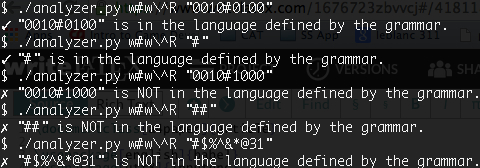
\includegraphics[width=1\textwidth]{string-reversestring_test.jpg}
\\
\paragraph{} The following grammar could not be represent with a simple expression as the previous grammars. The only explanation I can give is that this grammar accepts valid algebraic expressions in the form of "(SAS)" where S can either map to "(SAS)" again or it can map to a lower-case character or number. A can map to an algebraic operation such as +,-,/, and *.
\\
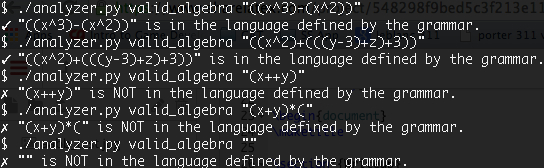
\includegraphics[width=1\textwidth]{valid-algebra_test.jpg}

\vspace{25mm}
\section*{Questions}
    \begin{enumerate}
        \item Why were those particular restrictions placed on the grammars?
        \paragraph{} The two restrictions mentioned at the beginning of this document were put in place to simplify the algorithm by a lot. The first rule states that all grammars must have rules with a terminal as their first character. The second rule ensures that no two rules for a single variable can start with the same terminal. This makes it easier because I didn't have to include any logic to determine which of the two rules to use; I could just look at the first character of the rule and assume that's what I would need (it disambiguates the problem for us).
\\ \\   \item If those restrictions weren't there, how would your program need to change?
        \paragraph{} The algorithm in my program for parsing a string would change quite a bit. I would need to somehow know which rules to choose if there were multiple with the same starting terminal and having a variable as the first character in a rule would change the part of my algorithm where I use the first character of a rule to determine which rule to push onto my stack. I wouldn't be able to compare the current input string to the first characters in the rules.
        
        \item What would happen if the grammar were ambigious?
        \paragraph{} It would be possible for my grammar to generate more than one left-most derivation which would be a lot harder to determine what the start of my string is always different and it'd therefore need be to read/compared differently to the stack.
        \item What other approaches might be used to tell if a string can be generated by a given grammar?
        \paragraph{}The only other way I could think of is recursively replacing each variable (starting with the start variable) with any of its rules until all of the variables have been replaced by terminals. The rules uses to replace the variables could be determined somehow by reading both ends of a string and seeing which rule contains each of those characters on its ends. This would be difficult because it would basically only work for rules that have an even amount of terminals surrounding their variables.
    \end{enumerate}

\section*{Additional Information}


\textbf{Repository:} https://github.com/maxmarchuk/Grammar-Analyzer

- Code will be attached as a zip file along with some sample grammar encodings. 


\end{document}
